\documentclass{article}
\usepackage{graphicx}
\usepackage[margin=1.5cm]{geometry}
\usepackage{amsmath}
\usepackage[colorlinks=true,urlcolor=blue]{hyperref}

\begin{document}
\twocolumn

\title{Midterm 1 Study Guide (in-class)}
\author{Prof. Jordan C. Hanson}

\maketitle

\section{Unit 0}

\begin{enumerate}
\item Which of the following represents the density of lead?
\begin{itemize}
\item A: 0.11 g cm$^{-3}$
\item B: 1.1 g cm$^{-3}$
\item C: 11 g cm$^{-3}$
\item D: 111 g cm$^{-3}$
\end{itemize}

\item If there are 2.2 lbs/kg, which of the following is equivalent to 100 lbs in kg?
\begin{itemize}
\item A: 220 kg
\item B: 100 kg
\item C: 45.5 kg
\item D: 10.5 kg
\end{itemize}

\item A train leaves Los Angeles Union Station for the San Francisco at 60 km/hr.  If the San Francisco is 600 km to the North, how long before the train reaches the destination?
\begin{itemize}
\item A: 1 hour
\item B: 10 hours
\item C: 15 hours
\item D: 24 hours
\end{itemize}

\item A \textbf{vector} is a physical quantity with a magnitude and a direction: $\vec{v} = v_x \hat{i} + v_y \hat{j}$.  The $v_x$ is the amount in the x-direction, and the $v_y$ is the amount in the y-direction.  The $\hat{i}$ and the $\hat{j}$ are \textbf{unit vectors}.  The $\hat{i}$ points in the x-direction, and the $\hat{j}$ points in the y-direction.  Each has length 1 and no units. (a) Let $\vec{v} = -2\hat{i} + 2\hat{j}$, and $\vec{w} = 2\hat{i} - 2\hat{j}$.  Draw each in a 2D coordinate system below. (b) What is $\vec{v} + \vec{w}$?  (c) What is $\vec{v} - \vec{w}$? \\ \vspace{3cm}

\item Suppose the location of an aircraft is described by a 2D coordinate system in which East corresponds to the postive x-axis, and North corresponds to the positive y-axis.  The plane takes off from the origin in a direction 45 degrees above the xy-plane heading North, with a speed of 200 km/hr.  (a) Determine the components of the velocity, and write it as a vector $\vec{v} = v_x \hat{i} + v_y \hat{j}$.  (b) What is the plane's location after 6 minutes?  (c) Five minutes into the flight, the plane's angle above the xy-plane changes to 0 degrees, and it also turns due East. The \textit{speed} remains 200 km/hr for another 6 minutes.  What is the final location? \\ \vspace{4cm}

\item Suppose the velocity of a Metro train is 40 km hr$^{-1}$ at $t=0$ seconds, and 60 km hr$^{-1}$ at $t=4$ seconds. (a) What is the acceleration in km hr$^{-1}$ s$^{-1}$? (b) What is the acceleration in m s$^{-2}$? \\ \vspace{2cm}

\end{enumerate}

\section{Unit 1}

\begin{enumerate}
\item Using the \textbf{\href{https://phet.colorado.edu/en/simulations/pendulum-lab}{Pendulum Lab Simulation}}, calculate the average value of the gravitational acceleration, $g$, from period and length data.  Use the formula $T = 2\pi\sqrt{L/g}$. List your measurements, and the average and standard deviation of $g$: \\ \vspace{4cm}

\item Consider the motion of the sytem depicted in Fig. \ref{fig:1}.  (a) From the given data, calculate the speed of the system at points P and Q. (b) Is the acceleration of the sytem positive or negative?  Estimate the acceleration. \\ \vspace{3cm}

\begin{figure}
\centering
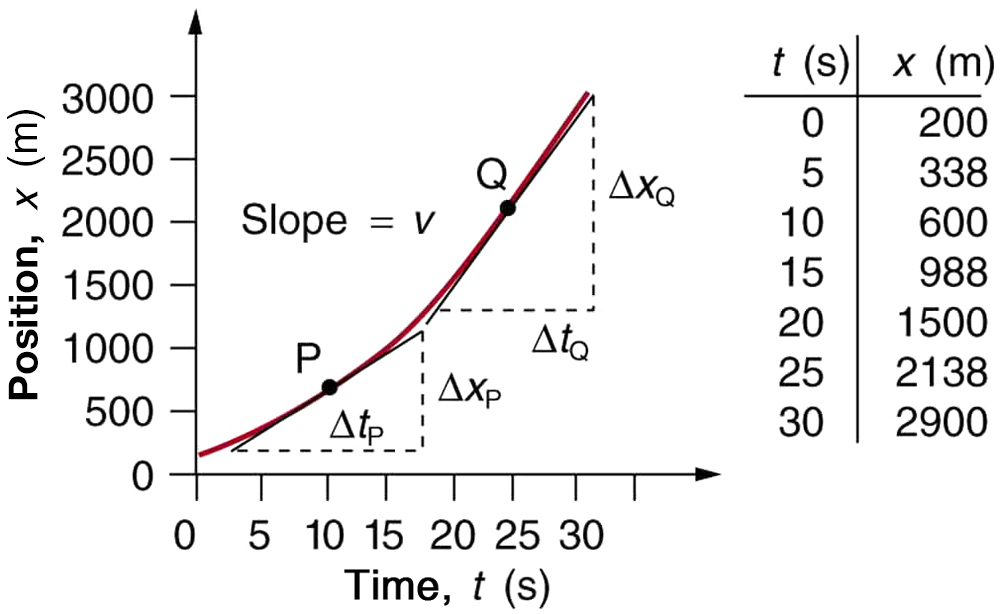
\includegraphics[width=0.4\textwidth]{slope2.jpeg}
\caption{\label{fig:1} A system moves with non-constant velocity.}
\end{figure}

\item Kilauea in Hawaii is the world's most continuously active volcano. Very active volcanoes characteristically eject red-hot rocks and lava rather than smoke and ash. Suppose a large rock is ejected from the volcano with a speed of 25.0 m/s and at an angle 35 degrees above the horizontal, as shown in Fig. \ref{fig:2}. The rock strikes the side of the volcano at an altitude 20.0 m lower than its starting point. (a) Determine the \textit{y-component} of the initial velocity of the rock.  (b) Determine the \textit{x-component} of the initial velocity. \\ \vspace{2cm}
\item Note that the vertical acceleration is $-g$. (a) Calculate the time it takes the rock to land. (b) Note that the horizontal acceleration is zero.  Determine the horizontal displacement of the rock from the top of the volcano when it lands. \\ \vspace{3cm}

\begin{figure}
\centering
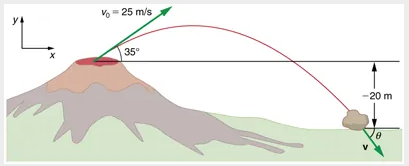
\includegraphics[width=0.49\textwidth]{volcano.png}
\caption{\label{fig:2} A volcano ejects a projectile.}
\end{figure}

\end{enumerate}

\section{Unit 2}

\begin{enumerate}
\item Using the \textbf{\href{https://phet.colorado.edu/en/simulations/hookes-law}{Spring Force Simulation}}, \textbf{graph} the applied force versus displacement for a system of two springs \textit{in parallel}, each with a $k$-value of 100 N m$^{-1}$.  If applied force is on the y-axis, and displacement is on the x-axis, what is the value of the slope, in N m$^{-1}$? \\ \vspace{3cm}

\item A 20,000 kg jet fighter lands on an aircraft carrier, moving at 108 km/hr. A tow cable grabs the aircraft and pulls it to a stop in 100 meters. (a) What is the average acceleration? (b) What force does the tow cable extert to stop the jet? \\ \vspace{3cm}

\item A rocket of mass $m$ is falling under the influence of gravity, but experiences a thrust force upwards $\vec{F}_t$, making the net force $\vec{F}_{\rm Net} = \vec{F}_t-\vec{w}$.  (a) Suppose the acceleration is $a = (k/m) - g$.  Write an expression for $\vec{F}_t$. (b) If the velocity at $t=10$ seconds is 10 m s$^{-1}$, and the velocity at $t=20$ seconds is 30 m s$^{-1}$, what is $k$? (c) What is the net force on the rocket? \\ \vspace{4cm}

\item Recall our lab activity in which we measured the coefficient of \textit{static} friction by placing a weight on an inclined index card, and varying the angle until motion was observed.  Using Fig. \ref{fig:3}, make an argument why this experiment measures the \textbf{maximum} force of static friction, and therefore the \textit{static} coefficient.  Is it possible to observe an angle larger than 45 degrees?

\begin{figure}
\centering
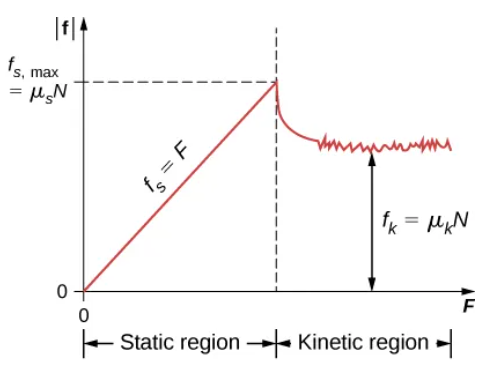
\includegraphics[width=0.333\textwidth]{friction_diagram.png}
\caption{\label{fig:3} Observed friction force versus applied force..}
\end{figure}

\item If a rubber eraser is placed on a physics textbook, and it begins to slide when the book is tilted to $\theta = 42$ degrees, what is the coefficient of static friction? \\ \vspace{2cm}

\item Design an experiment to measure the force of drag in air.  That is, design a process that would allow you to measure the value of $C$ in $F_{\rm D} = (1/2) C \rho A v^2$, assuming your system could reach terminal velocity.  (a) How would you record the data? (b) How would you measure the mass of the falling system?  (c) How would you measure the velocity?  (d) From the velocity data, how would you measure $C$? \\ \vspace{4cm}

\end{enumerate}

\section{Unit 3}

\begin{enumerate}
\item A boy pulls a 5-kg cart with a 20-N force at an angle of 30 degrees above the horizontal for a length of time. Over this time frame, the cart moves a distance of 12 m on the horizontal floor. (a) Find the work done on the cart by the boy. (b) What will be the work done by the boy if he pulled with the same force horizontally instead of at an angle of 30 degrees above the horizontal over the same distance? \\ \vspace{3cm}
\item Suppose a ball of mass $m$ is loaded onto a spring, and the spring is compressed by $\Delta x$. (a) Derive an expression for the initial speed of the ball if it is launched by the spring. (b) How high will the ball go above the launch point, if it has a mass of 50 grams, and the spring is compressed by 10 cm? \\ \vspace{3cm}
\item Design a spring-launcher that would launch the mass in the previous exercise a horizontal range of 10 meters. (a) How would you measure the k-value of the spring?  (b) How would you measure the launch angle? (c) How would you predict the range?
\end{enumerate}

\end{document}
